\documentclass[11pt, oneside]{article} 

\usepackage[parfill]{parskip} % Begin paragraphs with newline not indent
\usepackage{amssymb}
\usepackage{geometry}
\usepackage{graphicx}		
\usepackage{xspace}
\usepackage{listings}

\geometry{letterpaper}

\title{Messaging Layer Security (MLS)}
\author{TODO}

\newcommand{\protoname}{MLS\xspace}

\usepackage{todonotes}
\newcommand{\todokcg}[1]{\todo[inline,color=pink!60,author=Katriel]{#1}}
\newcommand{\todorlb}[1]{\todo[inline,color=blue!20,author=bifurcation]{#1}}

\begin{document}
\maketitle

\section{Overview}

The \protoname protocol enables a group of participants to

\begin{itemize}
\item derive a shared, authentic, symmetric key known only to the members of the group;
\item add new members to the group; and
\item remove members from the group.
\end{itemize}

We assume that each participant is provisioned with an \emph{identity key pair} which is used to compute and verify digital signatures.  In the course of the protocol, each participant will also have a Diffie-Hellman \emph{leaf key pair} that can change over time.

\subsection{Cryptographic Primitives}

An instantiation of \protoname requires the following cryptographic primitives:

\begin{itemize}
\item{A signature algorithm}
\item{A key agreement algorithm (referred to as a Diffie-Hellman or DH algorithm below)}
\item{A hash function used in creating Merkle trees}
\item{An injection $\iota$ from octet strings to DH key pairs}
\end{itemize}

\subsection{State}

A \emph{group} in the context of \protoname comprises a set of participants with shared state.  Each participant $\pi$ holds the following participant-specific data at a given time:

\begin{itemize}
\item{An \emph{index} $\pi.index$ that indicates the participant's position in the trees that define the overall group state}
\item{A fixed \emph{identity key} $\pi.ik$ that is used to sign messages}
\item{A variable \emph{leaf key} $\pi.lk$ that is used to derive shared secrets for the group}
\end{itemize}

The state of a group evolves through a series of numbered \emph{epochs}.  An epoch transition occurs when the set of participants in the group changes, either by adding or removing participants or by a participant changing its leaf key.

An MLS group is initialized at epoch 0 with a single participant, its creator.  The message interactions defined below then update the state of the group to add/remove participants or update leaf keys.

Each group is identified within an application by a static identifier $G.id$. At a given epoch $e$, the state of a group $G$ comprises the following data:

\begin{itemize}
\item A static, public \emph{group ID} $G_e.id$ that uniquely identifies the group within the scope of the messaging system
\item A Merkle tree $G_e.T_I$ over the identity keys of participants in the conference
\item A Merkle tree $G_e.T_L$ over the leaf keys of participants in the conference
\item A "ratchet tree" $G_e.T_R$ over the leaf keys of the participants in the conference
\item An \emph{epoch secret} $G_e.k$, the symmetric key derived by \protoname
\item A set of shared secret values derived from the epoch secret:
	\begin{itemize}
	\item A \emph{message root key} $G_e.k_m$ used for deriving keys to protect messages
	\item An \emph{update secret}  $G_e.k_u$ used updating leaf keys
	\item An asymmetric \emph{add private key} $G_e.k_a$ used adding members to the group
	\end{itemize}
\end{itemize}

The Merkle trees are used to verify participants' membership in the group, while avoiding the need to cache or transmit the full list of participants.  A participant must have the full participant list in order to remove participants, and a delete message has $O(N)$ size, but all other messages are of size $O(\log N)$.

Each participant caches a view of this state that is sufficient to generate and consume messages that update the group's membership.  A participant is added to the group by initializing a view of the state of the group.  A participant is removed by updating the group's secrets such that they are no longer known to the removed participant.


\section{Merkle Trees and Ratchet Trees}

\todorlb{Need to describe how to operate a balanced binary tree, and how to instantiate it for a Merkle tree or a ratchet tree}


\section{Group Key Management}

\protoname enables the following changes to group membership:

\begin{itemize}
\item{Addition of a participant, initiated by a group member}
\item{Addition of a participant, initiated by the new participant}
\item{Update of a leaf key for a participant}
\item{Remove a participant}
\end{itemize}

Each change is accomplished by sending a single message to the group.  We call these epoch-changing messages \emph{handshake messages}.

Each message is premised on a given epoch; it represents a change from epoch $n$ to a new epoch $n+1$.  If multiple messages are issued premised on the same epoch, only one can be applied.  If the underlying messaging system imposes a consistent ordering on messages (i.e., that all participants will process messages in the same order), then the participants can simply accept the first message delivered per epoch.  Rejected messages can be recalculated on the new epoch and resent.  

\todorlb{Some messages might not actually need to be bound to an epoch; as long as they are applied in the same order, the message carries enough information for participants to rebase on a new epoch, rather than the sender having to do the rebase.  I think this is true of group-initiated adds.}


\subsection{Participant State}

Each participant maintains the following state for a group:

\begin{itemize}
\item{A description of this participant's role in the group:
	\begin{itemize}
	\item{This participant's index in the group}
	\item{This participant's identity key}
	\item{This participant's current leaf key}
	\item{This participant's copath in the ratchet tree $G.T_R$}
	\end{itemize}
}
\item{A view of the global state of the group:
	\begin{itemize}
	\item{The current epoch number $e$}
	\item{The group ID $G.id$}
	\item{The Merkle identity tree $G.T_I$ (or a partial version)}
	\item{The Merkle leaf tree $G.T_I$ (or a partial version)}
	\item{The ratchet tree $G$ of the ratchet tree $G.T_R$ (or a partial version)}
	\item{The current message root key, update secret, and add key pair}
	\end{itemize}
}
\end{itemize}

A given participant view of the identity tree and leaf tree might be incomplete.  On initialization, a participant is provided the frontier of each tree, allowing it to compute the right edge and head of each tree.  Receiving add messages will allow it to compute additional branches of the tree to the right of its position, as well as new tree heads.  It will need to have the full lists of identity keys and leaf keys before generating a Delete message, but having the heads of these Merkle trees allows it to download these lists from an untrusted source.

The key management messages listed below serve to initialize new participants and synchronize state between current participants.

When the first participant in a group creates the group, it initializes its own state to reflect a group containing only itself.

\begin{itemize}
\item{index: 0}
\item{identity key: (participant identity key)}
\item{leaf key: (fresh private key)}
\item{ratchet copath: (empty)}
\item{epoch: 0}
\item{group ID: (set by participant)}
\item{identity tree: (one-node tree over participant identity key)}
\item{leaf tree: (one-node tree over participant leaf key)}
\item{ratchet frontier: (one-node frontier, (leaf, 1))}
\item{message root key: (random)}
\item{message update secret: (random)}
\item{message add key pair: (fresh key pair)}
\end{itemize}


\section{Prekeys}

To allow for asynchronous additions of new participants, both users and groups can publish \emph{prekeys} that the other side can use to perform an add operation.  Individual participants can use a \emph{group prekey} to add themselves to the group.  Members of the group can use a \emph{user prekey} to add a user to the group.  In both cases, once members of the group have processed the add message, they can begin transmitting messages under a key that is held by all group members.

\begin{verbatim}
struct {
    DHPublicKey pre_key;
    SignaturePublicKey identity_key;
    SignatureScheme algorithm;
    opaque signature<0..2^16-1>;
} UserPreKey;

struct {
    uint32 epoch;
    uint32 group_size;
    opaque group_id<0..2^16-1>;
    DHPublicKey update_key;
    MerkleNode identityFrontier<0..2^16-1>;
    MerkleNode leafFrontier<0..2^16-1>;
    DHPublicKey ratchetFrontier<0..2^16-1>;
} GroupPreKey;
\end{verbatim}

A UserPreKey message is a signed message, where the signing key is the identity key for the user and the payload of the message is an initial leaf public key for the user.  Thus, the consumer of a user prekey receives an identity key and a leaf key for the user in question, as well as a proof of possession of the identity key.

A GroupPreKey message contains a snapshot of the public aspects of the group state:

\begin{itemize}
\item{The current epoch number $e$}
\item{The group ID $G.id$}
\item{The current frontier of the identity tree $G_e.T_I$}
\item{The current frontier of the leaf tree $G.T_L$}
\item{The current frontier of the ratchet tree $G.T_R$}
\item{The current add public key $pk(G_e.k_a)$}
\end{itemize}

Note that although the GroupPreKey is unsigned, it is typically carried within a Handshake message that includes both a signature by a participant in the group and a proof of the signer's inclusion in the group.


\section{Handshake Messages}

Each handshake message is sent by a group member to inform other group members about a change in the group.  In addition to the information needed to accomplish the change, each handshake message includes a group prekey for the state of the group after the change, a signature by the sender's identity key, and a proof that the sender's identity key is included in the identity tree for the group ($G_e.T_I$).

\begin{verbatim}
enum {
    none(0), 
    user_add(1), 
    group_add(2),
    update(3),
    delete(4),
    (255)
} HandshakeType;

struct {
    HandshakeType msg_type;
    uint24 inner_length;
    select (Handshake.msg_type) {
        case none:      struct{};
        case user_add:  UserAdd;
        case group_add: GroupAdd;
        case update:    Update;
        case delete:    Delete;
    };

    GroupPreKey pre_key;

    uint32 signer_index;
    MerkleNode identity_proof<1..2^16-1>;
    SignaturePublicKey identity_key;

    SignatureScheme algorithm;
    opaque signature<1..2^16-1>;
} Handshake;
\end{verbatim}

The following illustration summarizes how the group secrets are updated by each message:

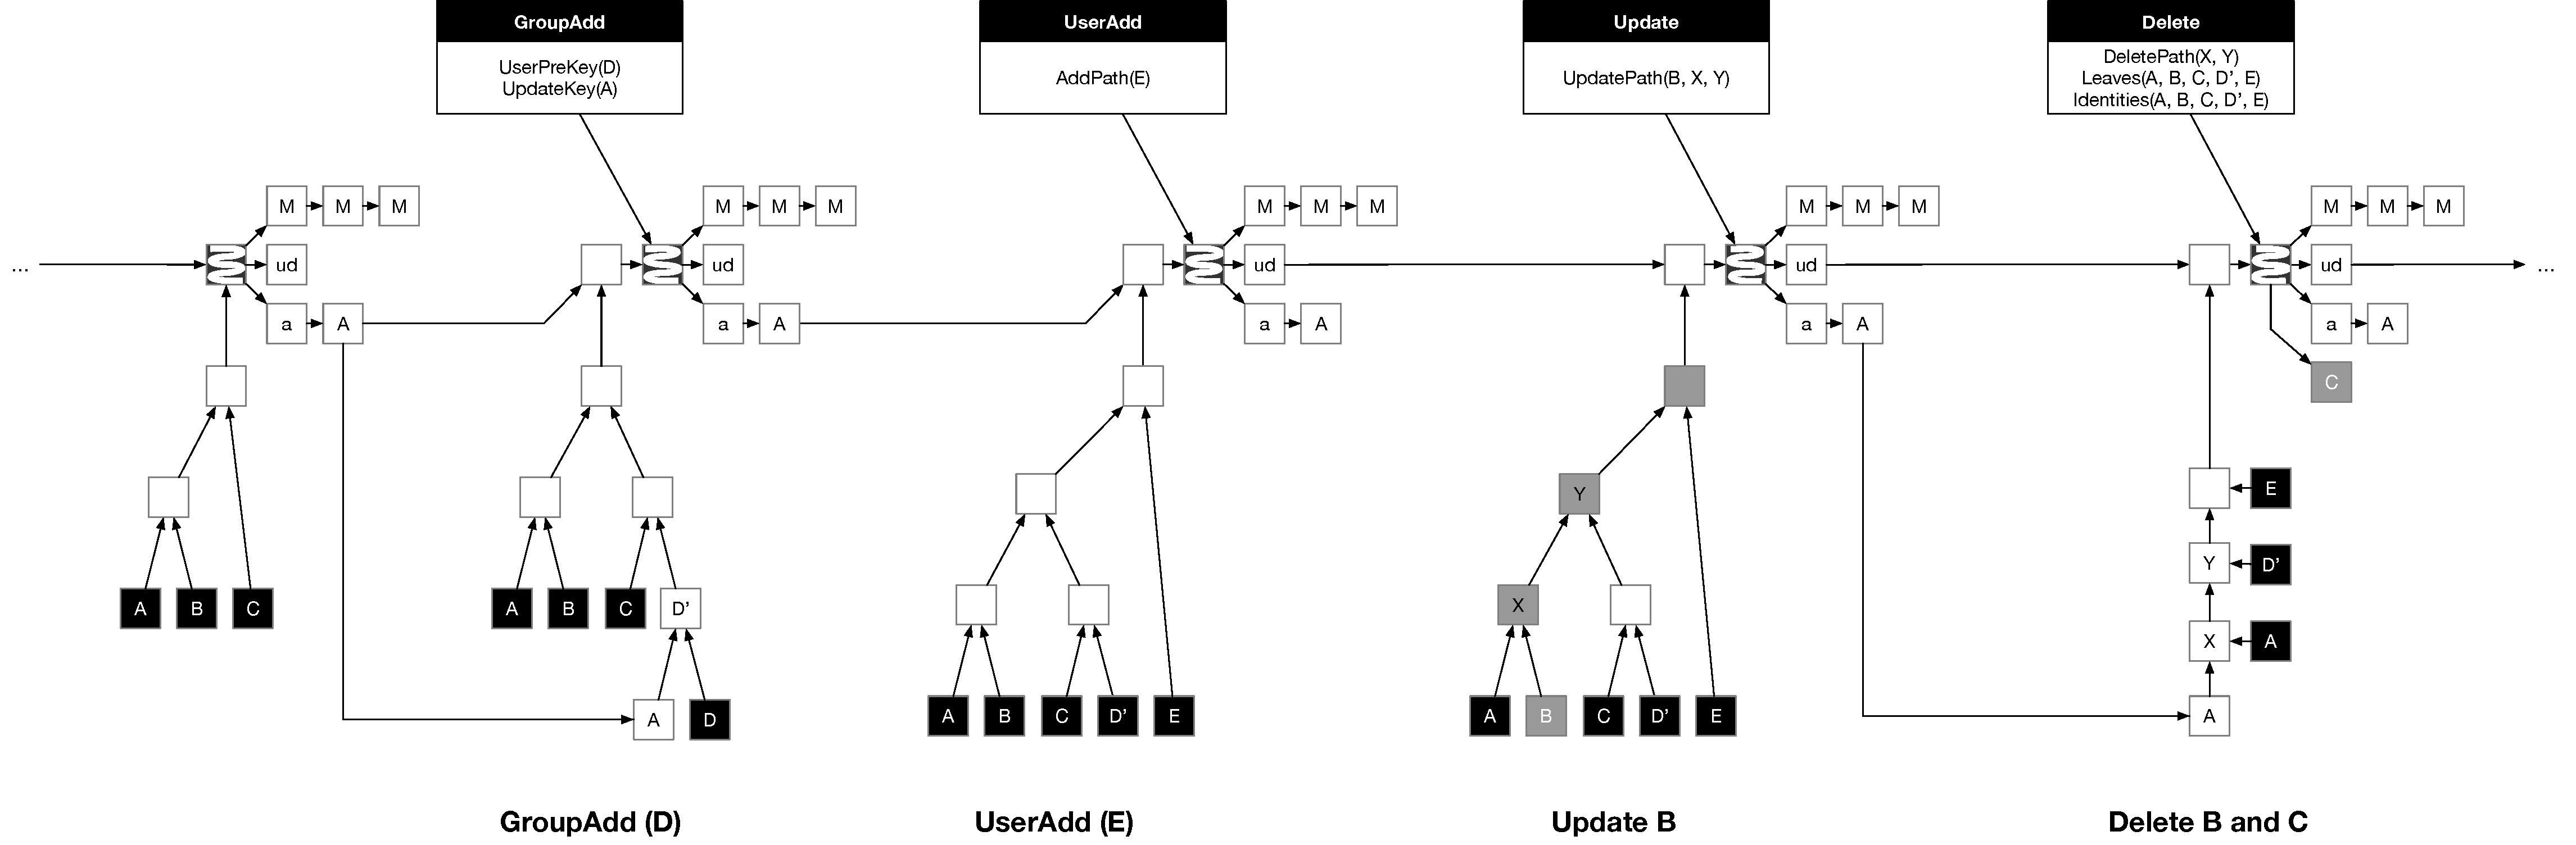
\includegraphics[width=\textwidth]{summary}


\subsection{Group-Initiated Add (GroupAdd)}

An GroupAdd message is sent by a group member to add a new participant to the group.  The contents of the message are simply the UserPreKey for the user being added.  

\begin{verbatim}
struct {
    UserPreKey pre_key;
} GroupAdd;
\end{verbatim}

A group member generates such a message by downloading a UserPreKey for the user to be added.

The added participant processes the message together with the private key corresponding to the user prekey to initialize his state as follows:

\begin{itemize}
\item{Compute the participant's leaf key pair by combining the prekey in the UserPreKey with the prior epoch add key pair}
\item{Use the frontiers in the GroupPreKey of the Handshake message to add its keys to the trees}
\item{Compute a new tree key from the ratchet tree and turn it into a key pair}
\item{Combine the tree key pair with the prior epoch's add key pair to get the epoch secret}
\item{Derive the group secrets for the epoch from the epoch secret}
\end{itemize}

An existing participant receiving a GroupAdd message first verifies the signature on the message, then verifies its identity proof against the identity tree held by the participant.  (This assures the recipient that the sender is a legitimate member of the group.)  The participant then updates its state as follows:

Existing group participants update their state as follows:

\begin{itemize}
\item{Compute the new participant's leaf key pair by combining the leaf key in the UserPreKey with the prior epoch add key pair}
\item{Update the group's identity, leaf, and ratchet trees with the new information}
\item{Compute a new tree key from the ratchet copath and leaf; turn it into a key pair}
\item{Combine the tree key pair with the prior epoch's add key pair to get the epoch secret}
\item{Derive the group secrets for the epoch from the epoch secret}
\end{itemize}


\subsection{User-Initiated Add (UserAdd)}

An UserAdd message is sent by a new group participant to add themselves to the group.

\begin{verbatim}
struct {
    DHPublicKey add_path<1..2^16-1>;
} UserAdd;
\end{verbatim}

A new participant generates this message using the following steps:

\begin{itemize}
\item{Fetch a GroupPreKey for the group}
\item{Use the frontiers in the GroupPreKey to add its keys to the trees}
\item{Compute the direct path from the new participant's leaf in the new ratchet tree}
\end{itemize}

An existing participant receiving a UserAdd first verifies the signature on the message, then verifies its identity inclusion proof against the \emph{updated} identity tree expressed in the GroupPreKey of the Handshake message (since the signer is not included in the prior group state held by the existing participant).  The participant then updates its state as follows:

\begin{itemize}
\item{Update trees with the descriptions in the new GroupPreKey}
\item{Update ratchet copath with the update path in the UserAdd message}
\item{Compute a new tree key from the ratchet copath and leaf; turn it into a key pair}
\item{Combine the tree key pair with the prior epoch's add key pair to get the epoch secret}
\item{Derive the group secrets for the epoch from the epoch secret}
\end{itemize}


\subsection{Leaf Key Update (Update)}

An Update message is sent by a group participant to update its leaf key.

\begin{verbatim}
struct {
    MerkleNode leafPath<1..2^16-1>;
    DHPublicKey ratchetPath<1..2^16-1>;
} Update;
\end{verbatim}

The sender of an Update message creates it in the following way:

\begin{itemize}
\item{Generate a fresh leaf key pair}
\item{Compute the direct path for its public key in the current leaf tree $G_e.T_L$}
\item{Compute its direct path in the current ratchet tree $G_e.T_R$}
\end{itemize}

An existing participant receiving a Update message first verifies the signature on the message, then verifies its identity proof against the identity tree held by the participant.  (This assures the recipient that the sender is a legitimate member of the group.)  The participant then updates its state as follows:

\begin{itemize}
\item{Update the cached ratchet tree by replacing nodes in the direct path from the updated leaf with the corresponding nodes in the Update message}
\item{Perform the same update on the leaf tree}
\item{Compute a new symmetric tree key from the ratchet tree and the local leaf key}
\item{Combine the tree key with the prior epoch's update secret to get the epoch secret}
\item{Derive the group secrets for the epoch from the new epoch secret}
\end{itemize}


\subsection{Removal of Participants (Delete)}

A delete message is sent by a group member to remove one or more participants from the group.

\begin{verbatim}
struct {
    uint32 deleted<1..2^16-1>;
    DHPublicKey path<1..2^16-1>;
    DHPublicKey leaves<1..2^16-1>;
    MerkleNode hashed_identities<1..2^16-1>;
} Delete;
\end{verbatim}

Unlike other messages, generating a delete message requires the sender to first have the full list of leaf keys and identity keys for all participants in the group, so that it can generate a secret value that is known to all participants except the deleted participants.  However, because each node caches trusted values for the roots of Merkle trees over these two data sets, the source from which the participant acquires these lists need not be trusted.

Given a list of nodes to be deleted, the sender of a Delete message generates it in the following way:

\begin{itemize}
\item{Construct a list of the leaf keys in tree order, with the deleted nodes omitted}
\item{Construct a "delete path" as a sequence of public keys of the same length as the list of leaf keys}
\item{Initialize a temporary private key from the current group add private key $G_e.k_a$}
\item{For each leaf key in the list of leaf keys:
	\begin{itemize}
	\item{Generate a new key pair using the temporary private key and the current leaf key}
	\item{Set the corresponding element of the delete path to the public key of this key pair}
	\item{Set the temporary private key to the private key of the new key pair}
	\end{itemize}
}
\item{Copy the cached lists of leaf keys and hashed identity keys to the Delete message}
\end{itemize}

An existing participant receiving a Delete message first verifies the signature on the message, then verifies its identity proof against the identity tree held by the participant.  (This assures the recipient that the sender is a legitimate member of the group.)  The participant then updates its state as follows:

\begin{itemize}
\item{Verify the list of leaf keys in the message against the root of the current leaf tree}
\item{Verify the list of hashed identity keys in the message against the root of the current identity tree}
\item{Construct a list of the leaf keys in tree order, with the deleted nodes omitted}
\item{Find the public key in the delete path corresponding to the highest index less than this node's index}
\item{Compute a new key pair by combining this node's leaf key with the previous public key in the delete path}
\item{For each leaf key to the right of this node, combine the leaf key with the generated private key to get a new key pair}
\item{For the last leaf key, do not generate a new key pair, but keep the output of the DH operation directly as a "delete secret"}
\item{Combine the delete secret with the prior epoch's update secret to get the new epoch secret}
\item{Derive the group secrets for the epoch from the new epoch secret}
\item{In the identity tree, replace the deleted nodes with empty nodes}
\item{In the leaf tree and ratchet tree, replace the deleted nodes with the new delete key pair}
\end{itemize}

After being deleted, a participant will still be able to compute the root of the ratchet tree on subsequent adds and updates.  However, it will no longer be able to compute the epoch secrets for future epochs -- they will depend on the delete secret computed above, which the deleted participant does not have access to.  A deleted participants ability to compute tree keys will be destroyed once its sibling updates its leaf key, at which point the root of the ratchet tree will be based on the delete key pair, which is not known to deleted participants.

\end{document}  








































